\documentclass[a4paper,fleqn]{article}
\usepackage{iemss}
\usepackage{times}
\usepackage{graphicx}
\usepackage{natbib}
\bibpunct{[}{]}{;}{a}{,}{,~}
\usepackage{multirow}
\usepackage{float}
\usepackage{subfig}
\pagestyle{IEMSSheadings}
% Text to appear in the header of the pages
\IEMSShead{Stefanescu et al. / Galeras}

\newcommand{\Deg}{$^{\circ}$}
\newcommand{\Pic}[2][0.85]{\begin{center}\includegraphics[width=0.8\textwidth,height=#1\textheight,keepaspectratio]{#2}
 \end{center} }



\title{Impact of DEM uncertainty on TITAN2D flow model output, Galeras
  Volcano, Colombia}

%Authors Names and Affiliations:  Two spaces below the title, 10 pt
%Times Roman, Upper and Lower Case, underline author presenting
%paper and  provide his/her email address
\author{\underline{E.R. Stefanescu} \address[A1]{\it{Department of Mechanical \& Aerospace Engineering, University at Buffalo, SUNY,
Buffalo,NY 14260 , (ers32@buffalo.edu, abani@buffalo.edu)}}, 
M. I. Bursik\address[B1]{\it{Dept. of Geology, University at Buffalo, SUNY,
Buffalo,NY 14260 , (mib@buffalo.edu, gcordoba@buffalo.edu, mfs@buffalo.edu)}}, G. Cordoba \addressmark[B1],\address[D1]{\it{Universidad de Nari\~{n}o, Colombia}}, A.K. Patra \addressmark[A1], D.C. Pieri \address[C1]{\it{Jet Propulsion Laboratory, Caltech, Pasadena, CA, 91109 USA, (dave.pieri@jpl.nasa.gov)}} and M.F. Sheridan\addressmark[B1] }


\begin{document}

\begin{abstract}
  In this paper we study the impact of errors and uncertainties in
  digital elevation models on the analysis of hazardous mass flows at
  Galeras volcano in Colombia.  The increasing use of computer models
  and software has made it imperative that the effect of errors in
  digital elevation models which crucially determine the flow
  characteristics be quantified. We illustrate in this paper the
  significant effect of such errors and also attempt to correlate
  these to flow features.
\end{abstract}
\begin{keyword}
  granular flow, computer model, TITAN2D, Galeras, Colombia
\end{keyword}

\maketitle

\section{Background and Motivation}
Model-based hazard analysis is increasingly the dominant mode of
hazard analysis for large classes of hazards where sparse data (large
return time of hazard event, etc.)  preclude more observation-based
methods. Model outputs are unfortunately critically dependent on
inputs and parameters. For geophysical flows one critical input to
flow models is the digital elevation model (DEM) of the terrain over
which the flow needs to be studied. However, terrain is often poorly
represented by the DEM with a lot of uncertainty in the elevations
which are then magnified in derived quantities like slopes and
curvatures. 

Building on previous work \citep{stefanescu1}, we focus in this paper
on the effect of DEM uncertainty on geophysical mass flow computations
using the TITAN2D code \citep{Patra2005}. Using Galeras volcano as a test case we
examine the effect of DEM uncertainty by creating a model of the error
and sampling it to create an ensemble of possible terrains (see
\citet{stefanescu2} for description of procedure). The flow simulation
is then run on every member of this ensemble.  Statistics on suitable
flow features like maximum flow depth can be used to quantify the
effect of errors and uncertainties in DEMs. These can also be compared
to terrain features to judge if particular terrain features lead to
additional sensitivity in flow computations --- thus requiring greater
care in model-based hazard analysis.

Computational models, such as TITAN2D are potentially valuable tools
for assessing the extent of potential flows and understanding their
dynamics at Galeras. There are several towns and villages on the
slopes of the volcano that could benefit from a detailed understanding
of potential pyroclastic flows and lahar hazards. In the absence of more detailed geological
records, this assessment can best be advanced by computational
modeling. However, for the outcomes to be sufficiently accurate for
public safety applications the models must appropriately represent the
physics of the flows, produce robust and accurate solutions of the
equations, and the effect of topographic uncertainty on model
performance should be evaluated.

\subsection{Why Galeras?}

Galeras Volcano (elevation 4,276 meters), located in southwestern Colombia (1\Deg 13.31' N and 77\Deg
21.68' W), is one of the most active volcanoes on the world
\citep{hurtado_1997}. Nearly 400,000 people currently live near the
volcano; 10,000 of them reside within the zone of high volcanic hazard
(ZAVA abbreviated in Spanish). Pyroclastic flows pose a major hazard
for this population. The current period of activity that began in 2004
presents a serious problem for all stakeholders: decision makers,
scientists, public safety officials, and general population.
Computational modeling has the potential to provide useful information
for hazard assessment and risk mitigation.  However, there is a need
to evaluate the validity of the modeling and the quality of the DEMs
available for use in such modeling.
 

Galeras  is an important volcano for
computational flow modeling from both risk management and scientific
perspectives \citep{calvache1997}. Forecasts of volcanic explosions
using various geophysical tools \citep{narvaez_1997} have occasionally
brought public warnings to a high level of alert during the past 20
years. When the alert reaches the highest level, the public are urged to evacuate some
local areas; this occured  as recently as January, 2010. The worst event at Galeras
occurred in 1993, when an eruption killed 9 scientists and journalists
\citep{baxter1997}.


The topography of the volcano presents a problem for creation of a
good DEM. The irregular morphology on a small scale, with steep slopes,
narrow channels, deep gorges and abrupt cliffs poses problems for the
creation of accurate GPS and topographic models of the volcano
\citep{ordones_2000}. In addition, the current flow hazard map at
Galeras is mainly based on the sparse geological record
\citep{calvache_1990a}. Dense vegetation, deep erosion, successive
deposits of lava and pyroclastic flows hinder the tracing of specific
deposits in the field.


 The diverse
effects of this landscape, as reflected in DEMs created by different
processes and of different scales, must be examined and quantified to
determine the level of confidence that can be placed in model
results. Galeras provides a wide range of topographic features that chalenge the use of computational flow models.


\subsection{Why uncertainty in DEM?}

 Digital elevation models (DEMs) uncertainties can be
generated by errors in the acquisition of topographic data and in the
interpolation methods used to build the elevation model. Hence, DEMs are representations of topography with
inherent errors that constitute uncertainty. Our current work
\citep{stefanescu1, stefanescu2} and the results of several others
\citep{Felix_Hebeler} show that DEM uncertainty affects the outcome
of models using them. However, the effects of DEM error on elevation
and derived parameters are often not evaluated by DEM users, and
methods to address DEM error have not been integrated with GIS
software packages \citep{Wechsler2006}. 

Spatial autocorrelation was identified as a significant feature of
DEMs, thus conditional simulations based on characterizing the degree
of autocorrelation have been used as an approach for error modelling
\citep{Goodchild_1992}.  To assess the effect of DEM uncertainty on a
geophysical model the following procedure was executed: (A) build an
elevation uncertainty model, (B) propagate the uncertainty through the
geophysical model, (C) perform a visual evaluation of the
uncertainties and their impact on the model's output.

\section{Procedure for Evaluating Impact of  DEM Uncertainty }

In a companion paper \citep{stefanescu2}, we discuss the procedure for
propagation of uncertainty, including that in DEMs in analyzing
hazards at Mammoth Mountain, California, USA.  In this paper analyzing DEMs at Galeras volcano,
 two test DEMs at 30 m spacing were considered for our analysis. The SRTM
30m DEM was derived by spline interpolation from a 90m DEM of southern
Colombia using radar data collected in 2000, while the ASTER DEM was
calculated at the NASA/USGS Land Processes DAAC using orthorectified
imagery from 12 January 2010.  The ASTER dataset was used as a
surrogate for the ``true'' elevation while the SRTM dataset was used
in creating the error model (Fig.~\ref{fig1} (a), (b)). To find the
error in a given DEM dataset the elevation of a DEM may be subtracted
from the ``true'' elevation at a given location. The effect of
correlated DEM error was then investigated using stochastic
conditional simulation to generate multiple equally likely
representations of the actual terrain surface. A raster error surface
was then produced for each of the 64 random surfaces. The mean and
the standard deviation of model flow depth output  determined from
randomly drawn, spatially independent points scattered across the
surface were taken as being representative of the whole. Finally, the impact
of data uncertainty propagation on the flow and the geophysical
model are  assessed.

\section{TITAN2D and Flow Simulations}

The TITAN2D code combines numerical simulations of a natural
geophysical granular flow with digital data of the natural terrain. It
is based on a depth-averaged model for an incompressible granular
materia governed by Coulomb-type friction interactions
\citep{Savage1989}. TITAN2D performs flow simulations on a DEM of a
desired region, the simulation accuracy being highly dependent on the
level of the DEM resolution and quality. The TITAN2D model uses as a
driving force the component of gravity along the terrain. Thus, local
slopes derived from the DEM elevation data are critical.


In our study of DEM uncertainties using TITAN2D, we drew on four
parameters to set the bounds of the computational modeling of
pyroclastic flows (PFs): 1) internal friction angle, 2) basal friction
angle, 3) maximum volume of the flows, and 4) minimum volume of the
flows. We chose parameters for the TITAN flow models to bracket the
range of flow volumes and to be representative of the friction angles
that have been used by other researchers in their computational models.  The internal
friction angle has little effect on the output of the
flow models \citep{Keith, sheridan_2005}. Many TITAN users have chosen
values of internal friction for PFs that range between 15 and 37
degrees with values between 30 and 35 being the most frequent values used
\citep{Patra2005, murcia_2010}. For our study we used 35 degrees.  The
choice of a basal friction angle has a large effect on the flow
dynamics in the TITAN2D simulations \citep{Patra2005,
  stinton_2006}. Factors that could affect the choice of basal
friction include the volume of the flow, the type of the PF, the
nature of the substrate and the amount of
channelization. \citet{murcia_2010} list the basal friction values
chosen by TITAN2D users; they range between 5 and 28 degrees; the mean
value being about 15 degrees. For this study we used a basal friction
angle of 21 degrees, similar to that for TITAN models of large PFs at
Pico de Orizaba, Mexico \citep{sheridan_2010}.
 
Volumes of pyroclastic flows at stratovolcanoes typically cover a few
orders of magnitude. The volume values in this study bracket the range
of possible PFs at Galeras. According to \citet{calvache_1990a},
Galeras volcano produced 5 large pyroclastic flow eruptive episodes;
an historic eruption in 1866, and prehistoric events in 1100, 2300,
2900, and 4500 yBP.  The total deposit volumes of these episodes range
from $1.1 \times 10^6$ to $8.9 \times 10^6$ $m^3$. Of course the deposits of
each episode could include as few as 1 flow but more likely they contain many flows. Thus, our choice of volumes ranges from $1.6 \times 10^5$ to $2.5
\times 10^6 m^3$, because of the high probable likelihood of many small occurring within the studied terrain.

We located the starting point of the flows at 239261 m easting and
132918 m northing based on locations of previous vents. A
rectangular area of approximative 40 $km^2$ was defined around
the vent within the available DEMs.  The shape of the initial failure
is a paraboloid for which the initial  thickness is
$h_{max}= 10m$ high for the smallest flows and $h_{max} = 100m$ high for the largest flows.
 

Following the technique
outlined in the companion paper \citep{stefanescu2}, realizations of
the terrain surfaces were created and used as representations of the
topography in the modeling. The correlogram for the data was calculated to determine the range of spatial dependence of elevation points
 using Grass GIS functions. We found that this spatial dependence persisted to a distance of 2500 meters. To determine the probability distribution function (PDF)
 for the stochastic simulation, 91 sets of spot locations were selected from the area covered, each set containing 91 points, all pairs of points were separated 
 by more than 2500 meters. For each set, PDF statistics were derived.
The random field parameters were chosen
after testing more than 400 random field parameters. The combination
which resulted in the smallest difference between the error model
correlogram and the random field occurs when the minimum distance of
spatial independence, $D =2600$; the distance decay, $E = 0.8$, and
the filter parameter, $F =400$.  

\section{Discussion and Conclusions}

One of the output files produced by TITAN2D contains the maximum flow
depth over the entire simulated time at each grid point.  We use this
file in creating flow maps for a single particular run, and the maximum
flow depth of all 64 simulations for both low and high volume flows
(Fig.~\ref{fig2} (a), (b), Fig.~\ref{fig3} (a), (b)). These figures demonstrate large differences between small and large initial volumes.


  Next, we
investigated the best way to specify how the TITAN2D output
varies as a function of the DEM input, and if it is possible to
predict the flow using only a data-driven statistical model
without running the geophysical model. For this, we
examinated flow depth at a particular location on the terrain
surface for all simulations (Fig.~\ref{fig4} (a), (b)).  A visual
inspection of Figure ~\ref{fig4} shows that a linear or second order (quadratic fit) can not be employed to
determine a relation between the terrain (represented as $\epsilon$, corresponding to the random variable with
mean 0 and variance 1 used for creating terrain realizations) and the
flow. A randomness test with 5$\%$
significance level was performed and there was no sufficient evidence to reject the
null hypothesis that the maximum pile heights are random. 
The role of the fundamental physics based model is thus affirmed.
Furthermore, it is clear that the flow computations are very sensitive to
DEM errors and any attempt at model-based hazard analysis must include 
consideration of these errors.

It was demonstrated both analytically and empirically by
\citet{Hunter_Goodchild_1997} that errors in slope and aspect depend
on the structure of the spatial dependence. In this study the
dependence of the flow output on the (spatially dependent) slope and
curvature is investigated. In Fig.~\ref{fig3} (a), (b) the slope and
the curvature of the ASTER DEM are presented, with a range of 0\Deg to
70\Deg and -0.045 to 0.045 m$^{-1}$, respectively. It appears from
Figure~\ref{fig4} (a), (b) that low-volume flows are more ``stable''
relative to perturbations and irregularities in topography than are
high-volume flows.  In addition, at a 20\Deg slope for both high- and
low-volume flows, the geophysical model output appears to be most
sensitive to terrain changes.  However, this effect may be the result
of outlier sampling, as a 20\Deg slope is probably close to the most
common slope angle on a volcano \citep{BuPaPi05}.  Again, the maximum
in error at 0 curvature may result from outlier sampling, as on
average one may assume that the most frequently occurring curvature is
close to zero.


%\newcommand{\Pic}[2][0.85]{\begin{center}\includegraphics[width=0.8\textwidth,height=#1\textheight,keepaspectratio]{#2} \end{center} }
\begin{figure}[H]
    \begin{minipage}[b]{0.6\textwidth}
        \begin{tabular}{c}
        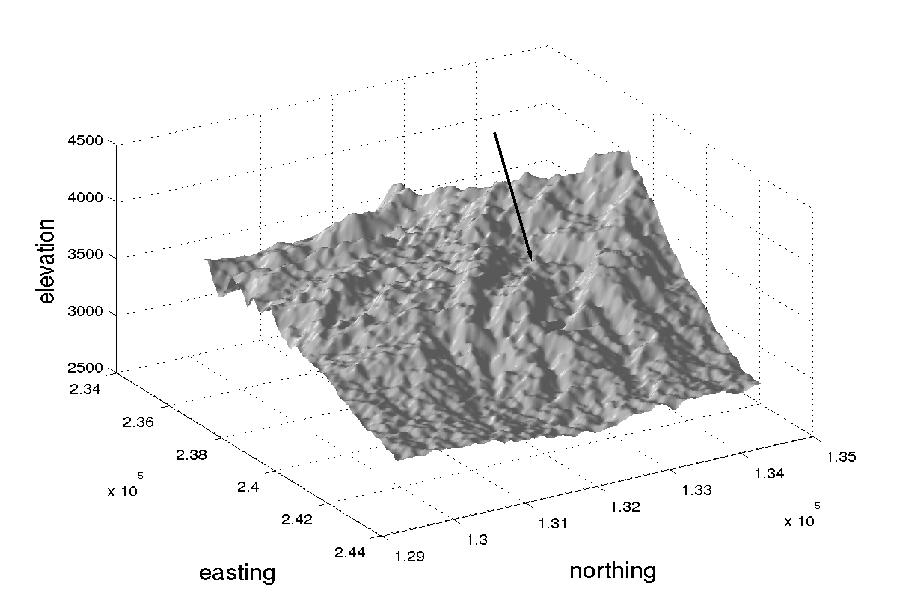
\includegraphics[width=7cm,height=8cm,keepaspectratio]{xfig_rot.jpg}\\
	%\Pic[0.3]{ASTER_DEM.jpg}	
        (a)
        \end{tabular}
    \end{minipage}
%\hfill
    \begin{minipage}{0.6\textwidth}
        \begin{tabular}{c}
	%\centering
        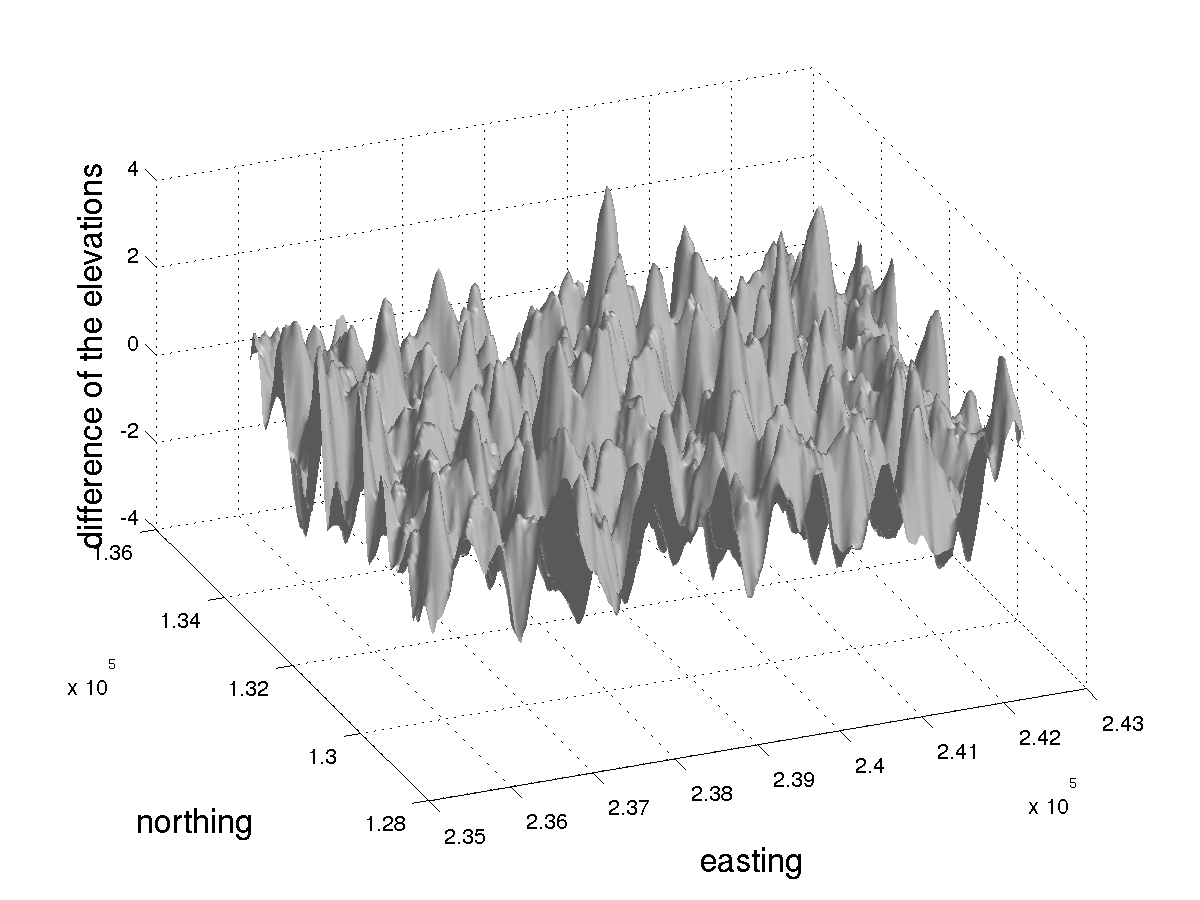
\includegraphics[width=7cm,height=8cm,keepaspectratio]{error3.jpg}\\
	%\Pic[0.3]{error.jpg}
        (c)
        \end{tabular}
    \end{minipage} 	
\caption{(a) Aster DEM in easting, northing and elevation coordinates; arrow points to the starting location of the flows. (b) Spatial distribution and magnitude of error}
\label{fig1}  
\end{figure}

\begin{figure}[H]
    \begin{minipage}[b]{0.6\textwidth}
        \begin{tabular}{c}
        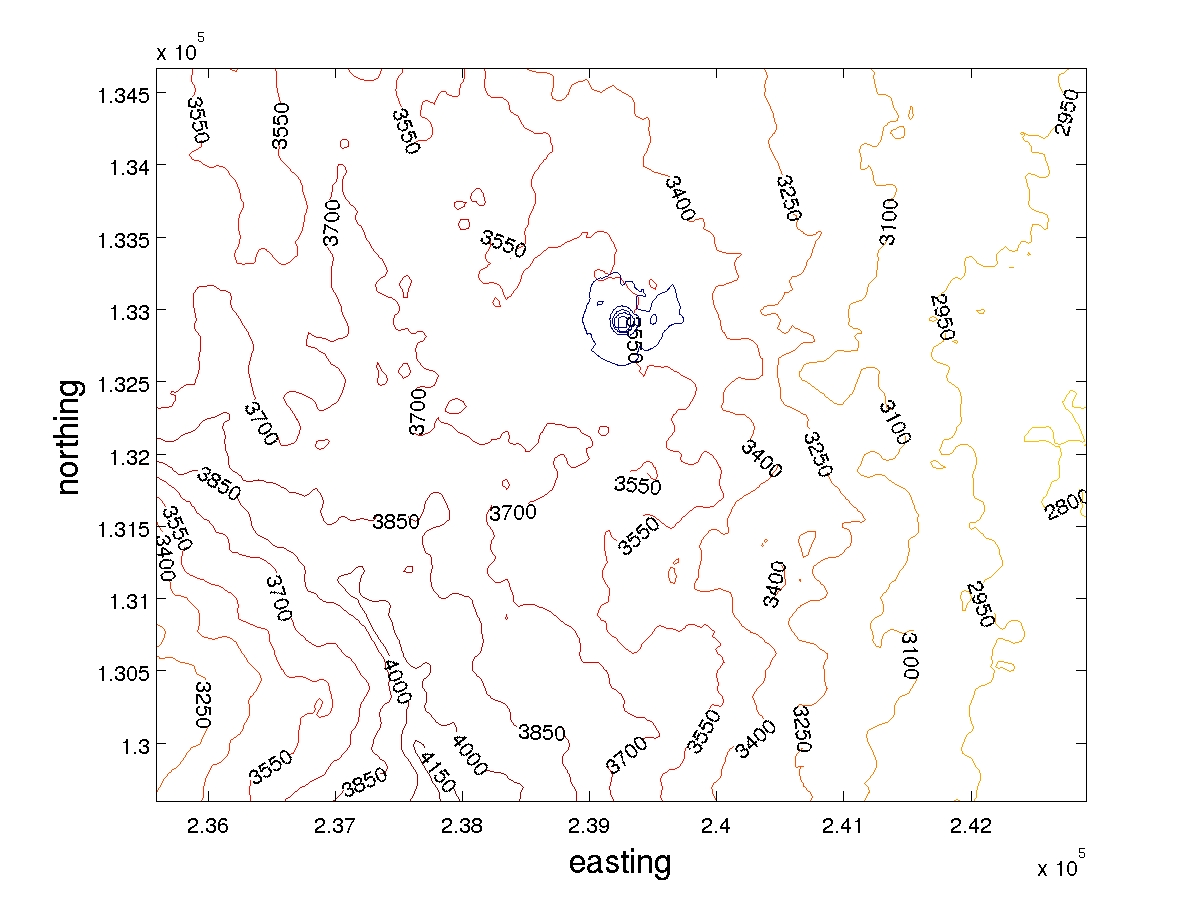
\includegraphics[width=9cm,height=8cm,keepaspectratio]{sample1_low_flow.jpg}\\
        (a)
        \end{tabular}
    \end{minipage}
%\hfill
    \begin{minipage}{0.6\textwidth}
        \begin{tabular}{c}
        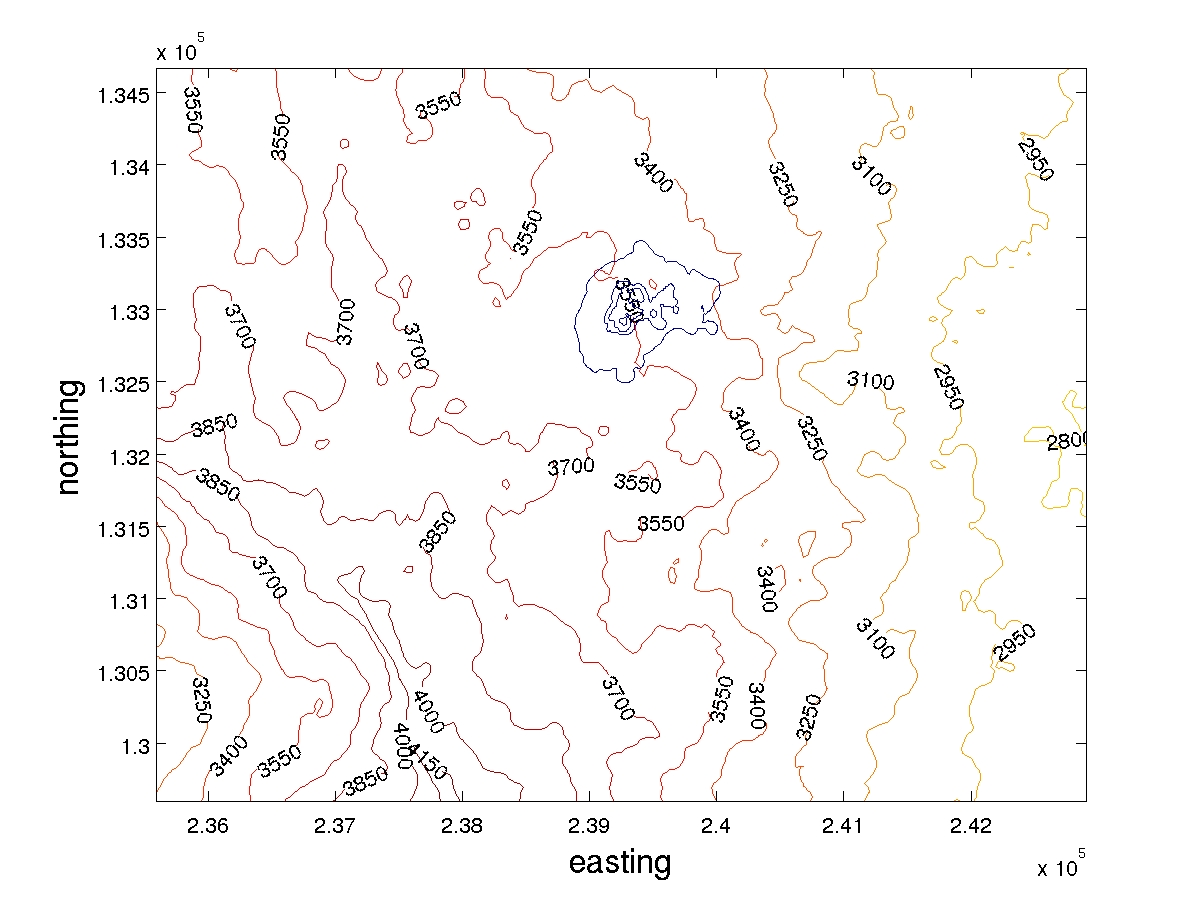
\includegraphics[width=9cm,height=8cm,keepaspectratio]{all_low_flow.jpg}\\
        (b)
        \end{tabular}
    \end{minipage} 
\caption{(a) Flow depth output for a single realization, low volume. (b) Maximum flow depth of all 64 realizations, low volume }
\label{fig2}  
\end{figure}

\begin{figure}[H]
    \begin{minipage}[b]{0.6\textwidth}
        \begin{tabular}{c}
        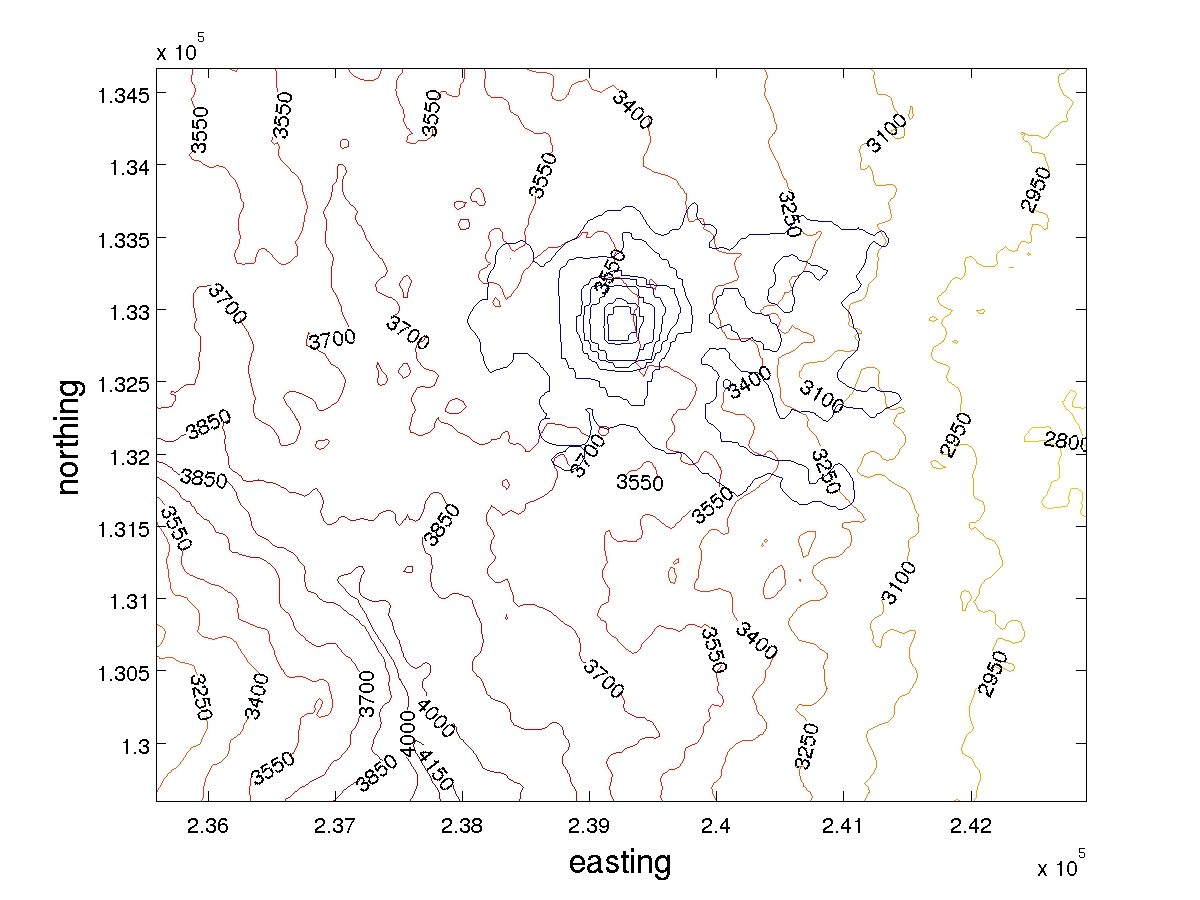
\includegraphics[width=9cm,height=8cm,keepaspectratio]{sample1_high_flow.jpg}\\
        (a)
        \end{tabular}
    \end{minipage}
%\hfill
    \begin{minipage}{0.6\textwidth}
        \begin{tabular}{c}
        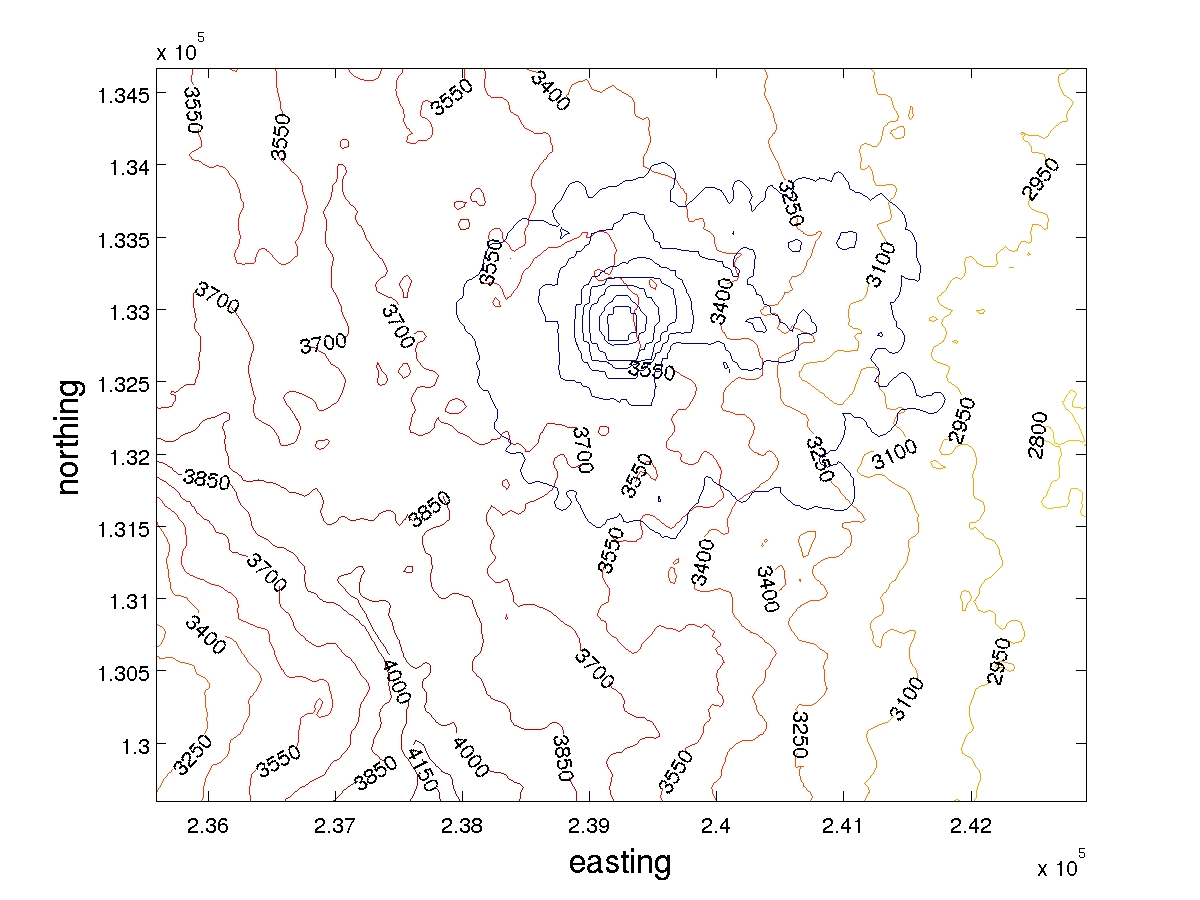
\includegraphics[width=9cm,height=8cm,keepaspectratio]{all_high_flow.jpg}\\
        (b)
        \end{tabular}
    \end{minipage} 
\caption{(a) Flow depth output for a single realization, high volume. (b) Maximum flow depth of all 64 realizations, high volume }
\label{fig3}  
\end{figure}

\begin{figure}[H]
    \begin{minipage}[b]{0.6\textwidth}
        \begin{tabular}{c}
        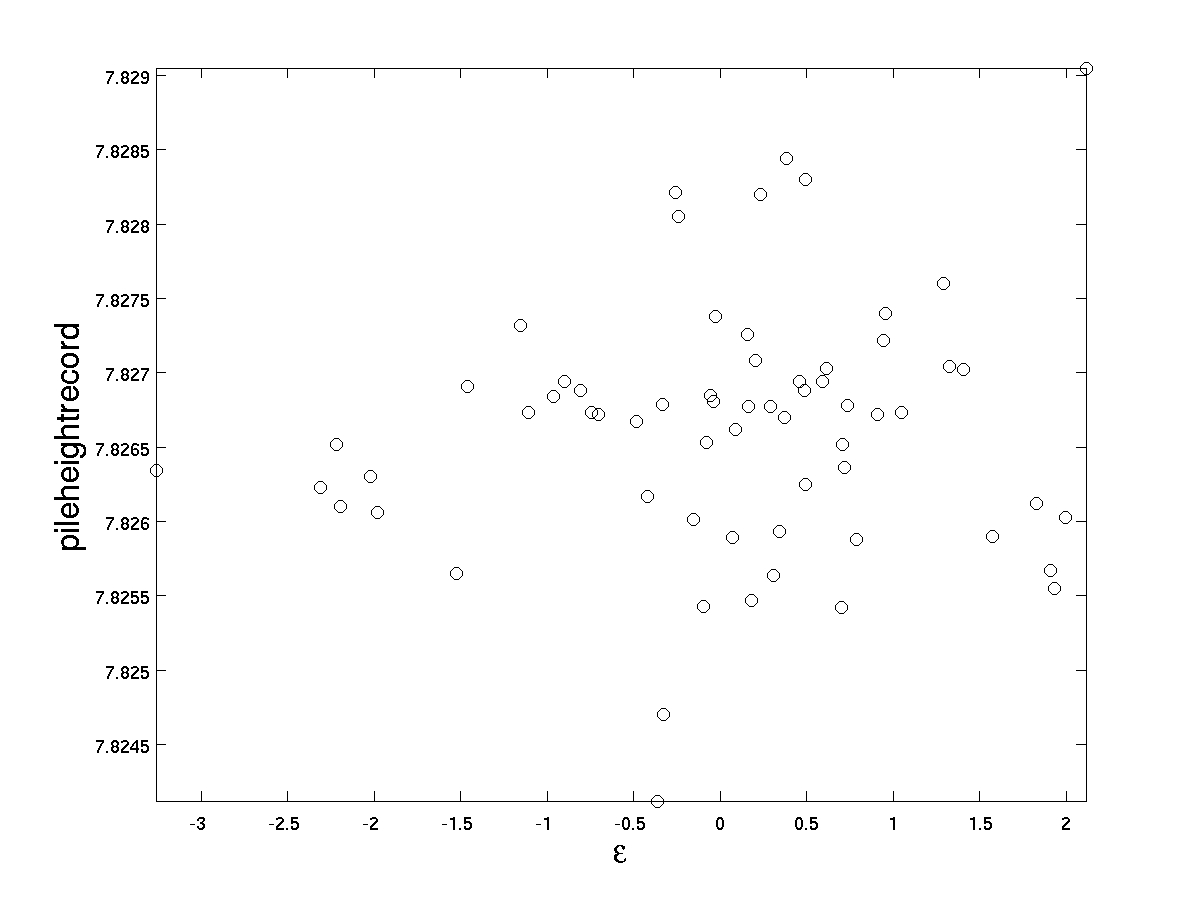
\includegraphics[width=9cm,height=8cm,keepaspectratio]{eps_vs_pile_low_vol.jpg}\\
        (a)
        \end{tabular}
    \end{minipage}
%\hfill
    \begin{minipage}{0.6\textwidth}
        \begin{tabular}{c}
        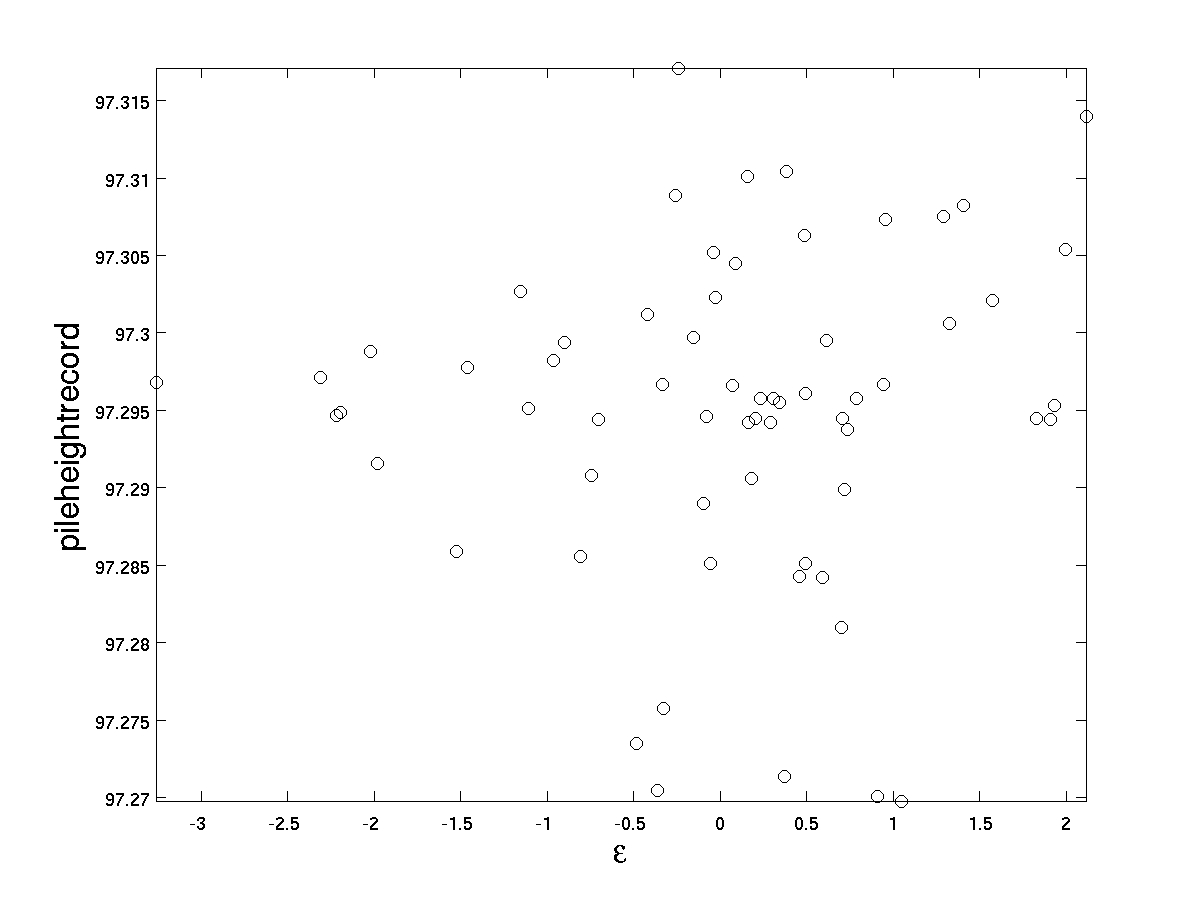
\includegraphics[width=9cm,height=8cm,keepaspectratio]{eps_vs_pile_high_vol.jpg}\\
        (b)
        \end{tabular}
    \end{minipage} 
\caption{The dependency of the flow depth on the terrain realizations at a specific location for, (a) low volume and (b) high volume}
\label{fig4}  
\end{figure}

\begin{figure}[H]
    \begin{minipage}[b]{0.6\textwidth}
        \begin{tabular}{c}
        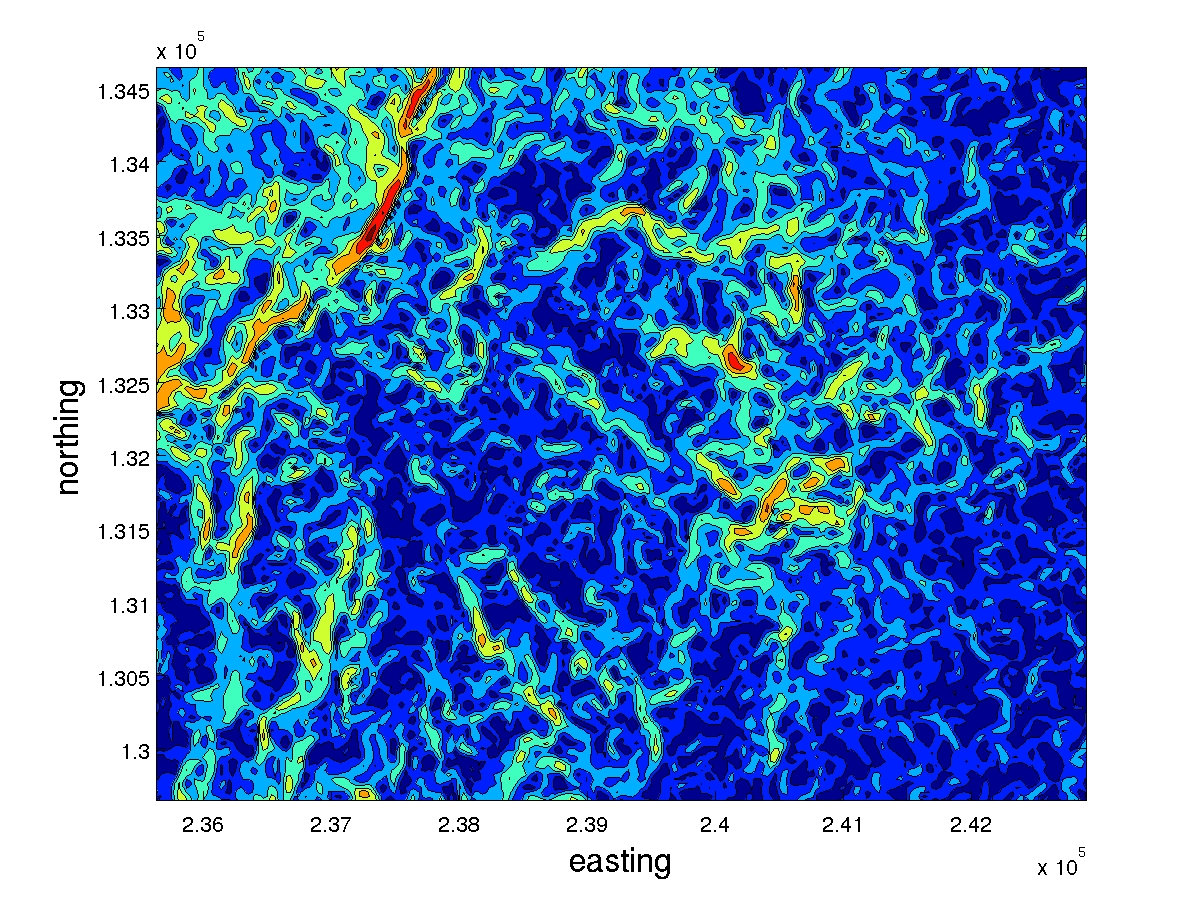
\includegraphics[width=9cm,height=8cm,keepaspectratio]{slope_profile.jpg}\\
        (a)
        \end{tabular}
    \end{minipage}
%\hfill
    \begin{minipage}{0.6\textwidth}
        \begin{tabular}{c}
        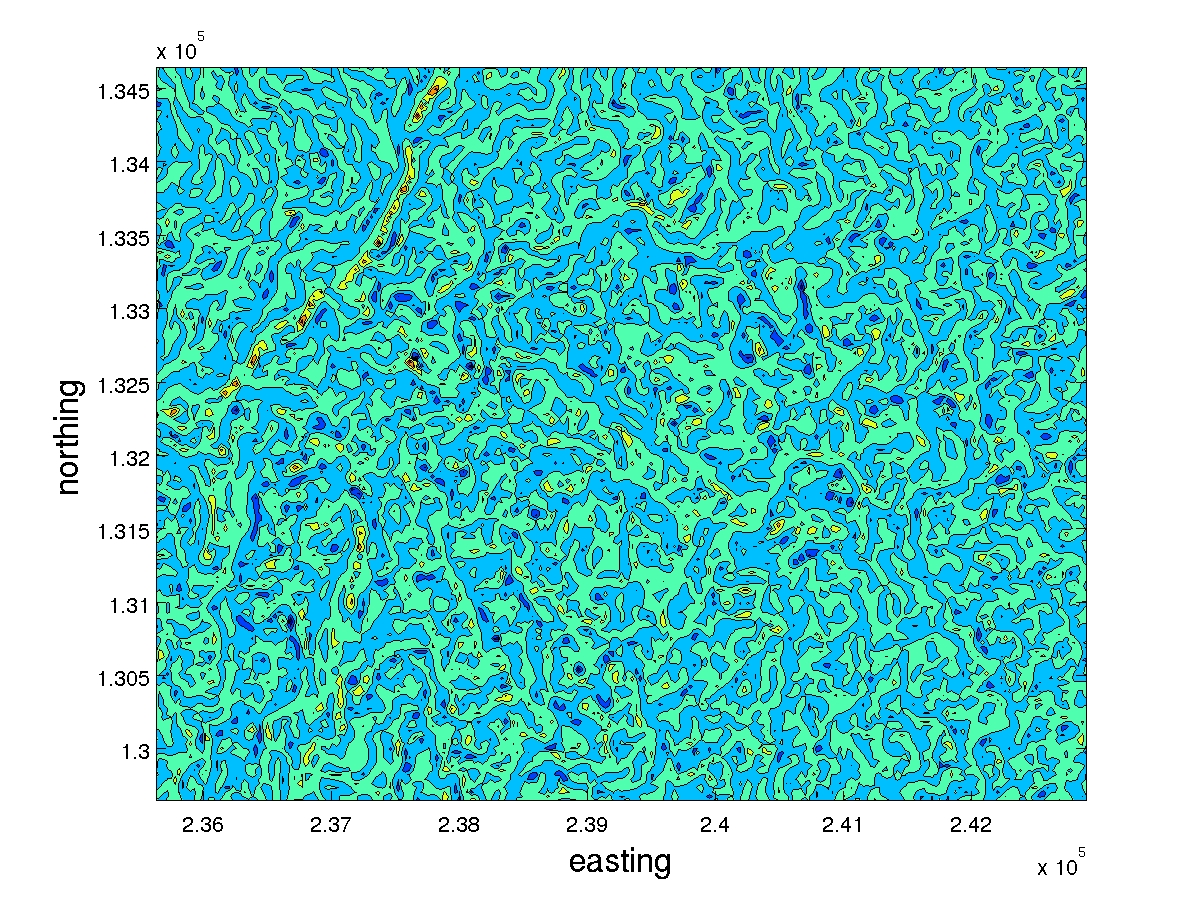
\includegraphics[width=9cm,height=8cm,keepaspectratio]{curvature_profile.jpg}\\
        (b)
        \end{tabular}
    \end{minipage} 
\caption{(a) Slope profile of the ASTER DEM. (b) Curvature profile of ASTER DEM}
\label{fig5}  
\end{figure}

\begin{figure}[H]
    \begin{minipage}[b]{0.6\textwidth}
        \begin{tabular}{c}
        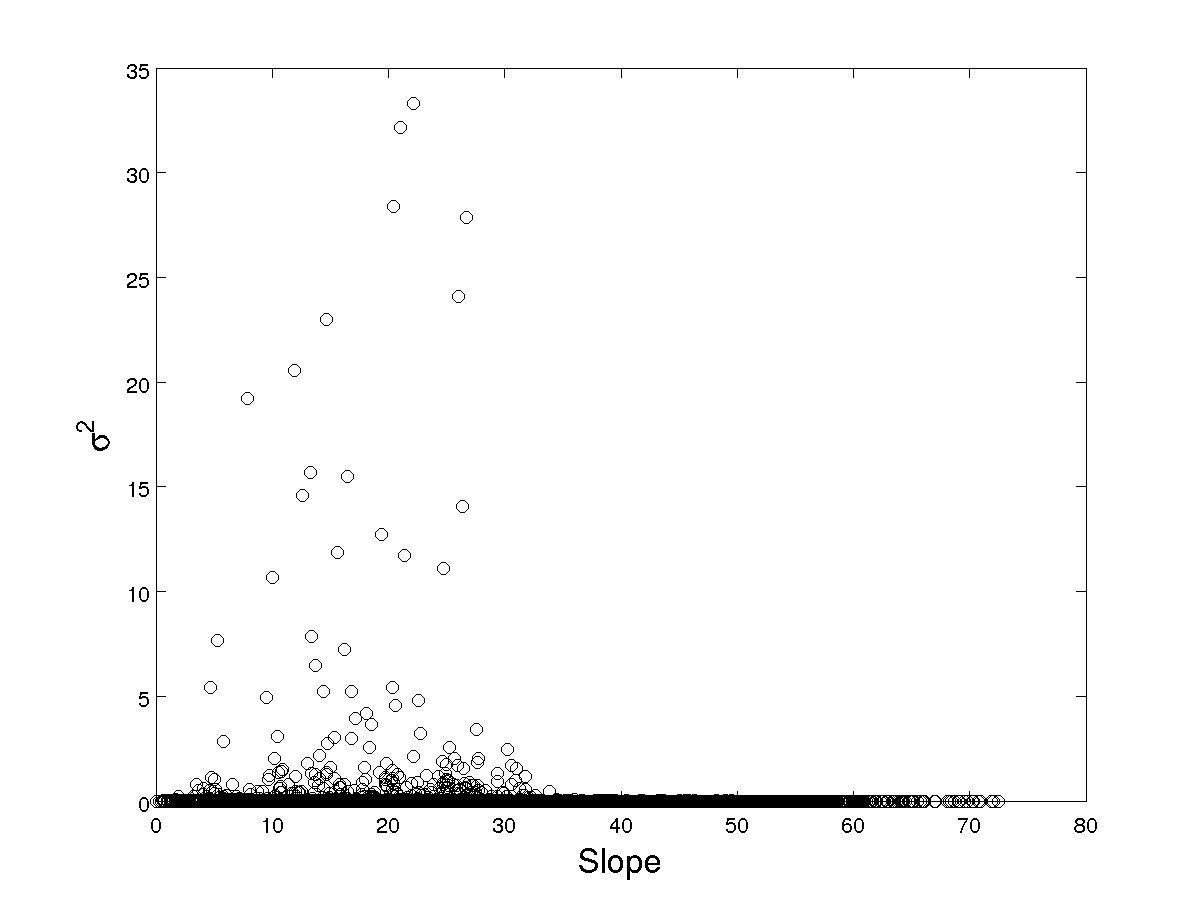
\includegraphics[width=9cm,height=8cm,keepaspectratio]{slope_vs_sigma2.jpg}\\
        (a)
        \end{tabular}
    \end{minipage}
%\hfill
    \begin{minipage}{0.6\textwidth}
        \begin{tabular}{c}
        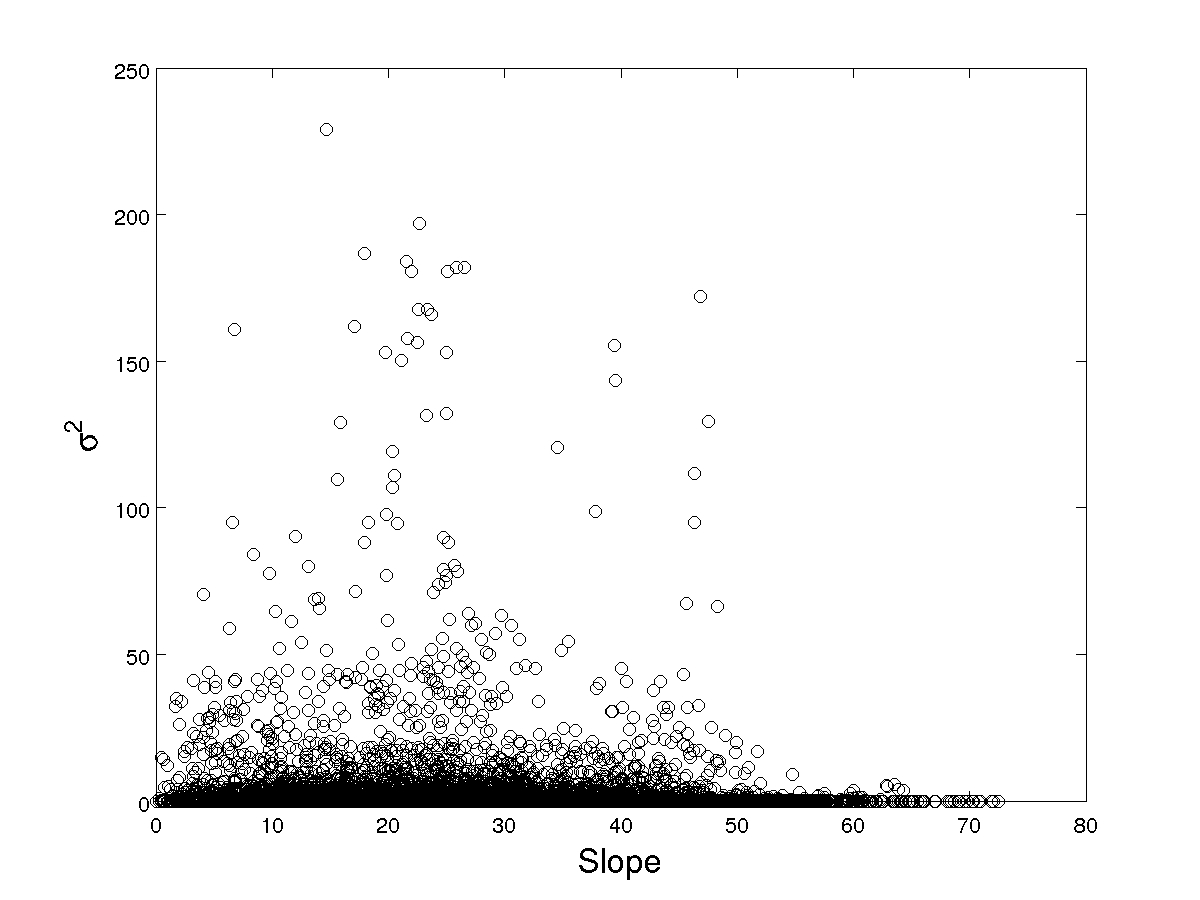
\includegraphics[width=9cm,height=8cm,keepaspectratio]{slope_vs_sigma2_high_vol.jpg}\\
        (b)
        \end{tabular}
    \end{minipage} 
\caption{Scatter plot showing the correlation of depth flow variance and slope for, (a) low volume and (b) high volume}
\label{fig6}  
\end{figure}
\begin{figure}[H]
    \begin{minipage}[b]{0.6\textwidth}
        \begin{tabular}{c}
        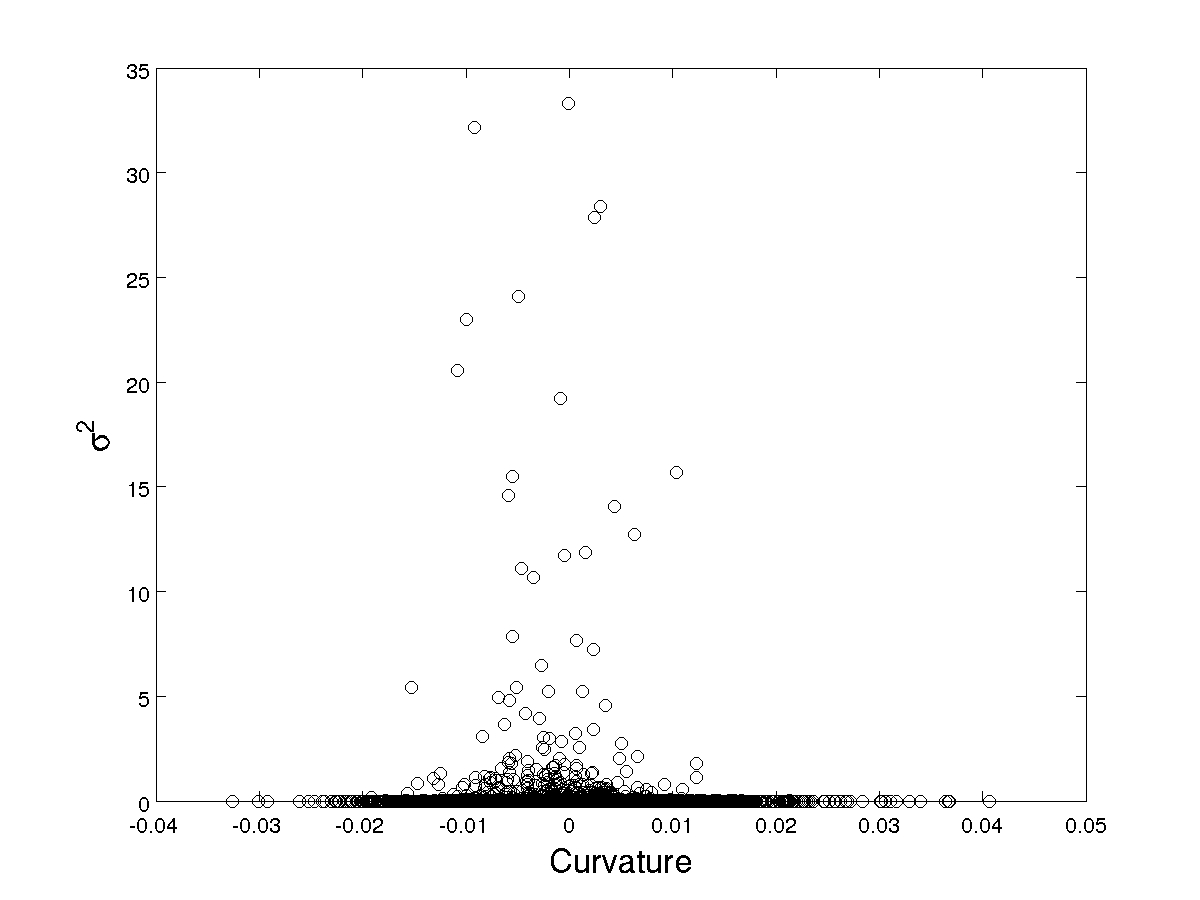
\includegraphics[width=9cm,height=8cm,keepaspectratio]{curvature_vs_sigma2.jpg}\\
        (a)
        \end{tabular}
    \end{minipage}
%\hfill
    \begin{minipage}{0.6\textwidth}
        \begin{tabular}{c}
        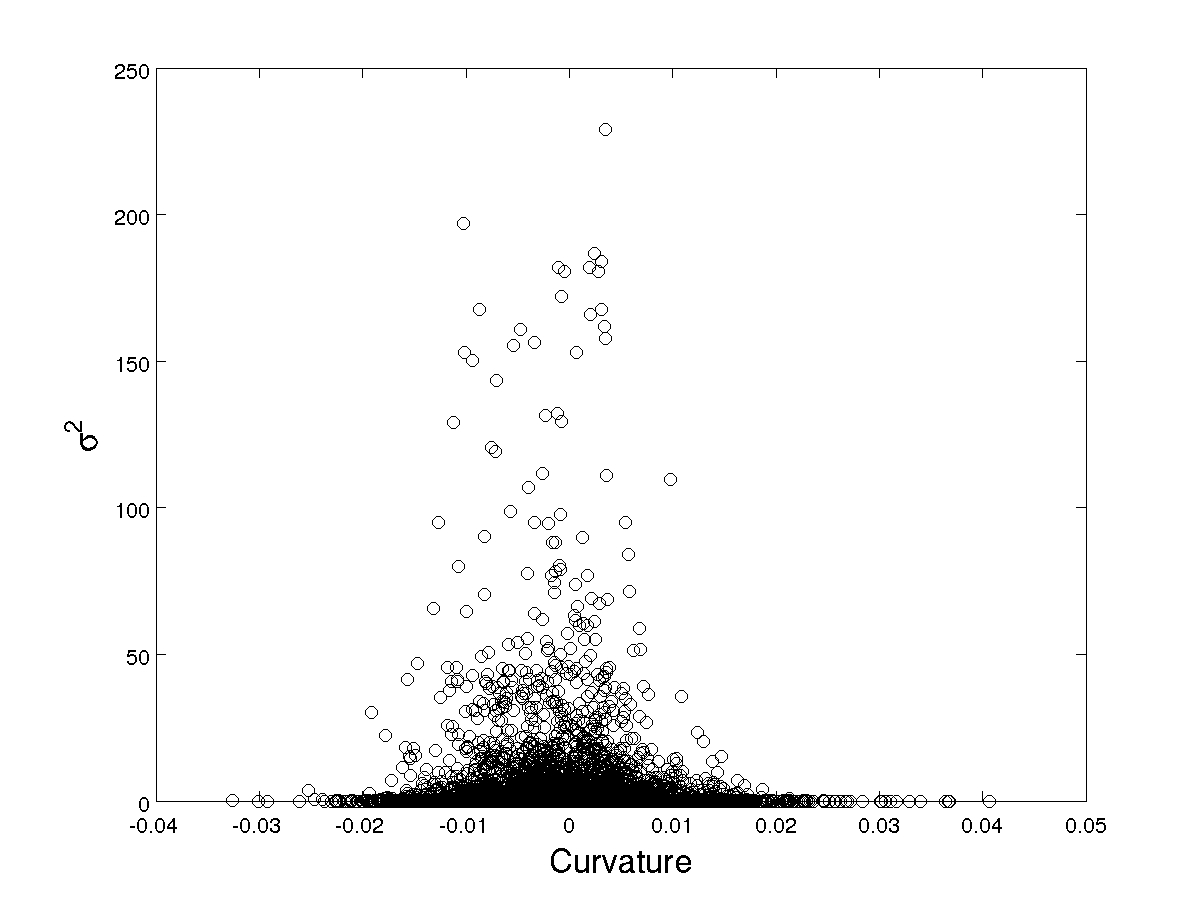
\includegraphics[width=9cm,height=8cm,keepaspectratio]{curvature_vs_sigma2_high_vol.jpg}\\
        (b)
        \end{tabular}
    \end{minipage} 
\caption{Scatter plot showing the correlation of depth flow variance and curvature for, (a) low volume and (b) high volume}
\label{fig7}  
\end{figure}




\section*{Acknowledgments}
This work was supported by NASA grant NNX08AF75G to study DEM
uncertainty on flow model output.  Referees are thanked for useful
comments and their time. The research of M.F. Sheridan and G. C\'ordoba was suported by NSF grant 0711497.


%%%%%%%%%%%%%%%%%%%%%%%%%%%%%%%%%%%%%%%%%%%%%%%%%%%%%%%%%%%%%%%%%
\bibliographystyle{iemss}
\bibliography{iemss_1.bib}
%%%%%%%%%%%%%%%%%%%%%%%%%%%%%%%%%%%%%%%%%%%%%%%%%%%%%%%%%%%%%%%%%

\end{document}
